% Generated from reviewed lane; compile via book/textbook.tex.
\clearpage

原书 PDF 页 318；印刷页码 305。

\href{source-images/pdf-318.jpeg}{原页图像}

\section{部分习题答案}\label{back-ux90e8ux5206ux4e60ux9898ux7b54ux6848}

\subsection{第 1 章}\label{back-ux7b2c-1-ux7ae0}

\textbf{1.} \(\delta\)。

\textbf{2.} \(0.02n\)。

\textbf{4.} \(1.05\times10^{-3}\)，\(0.215\)，\(10^{-5}\)。

\textbf{6.} \(\dfrac{1}{2}\times10^{-3}\)。

\textbf{9.} 边长误差小于 \(0.005\ \mathrm{cm}\)。

\textbf{11.} 不稳定，\(\varepsilon^*(y_{10})\approx\dfrac{1}{2}\times10^8\)。

\textbf{13.} \(0.3\times10^{-2}\)，\(0.834\times10^{-6}\)。

\subsection{第 2 章}\label{back-ux7b2c-2-ux7ae0}

\textbf{2.} \(5x^2/6+3x/2-7/3\)。

\textbf{3.} \(-0.620\,219\)，\(-0.616\,707\)。

\textbf{4.} \(1.06\times10^{-8}\)。

\textbf{5.} \((10+7\sqrt{7})/27\)。

\textbf{8.} \(h\leqslant0.006\)。

\textbf{9.} \(\Delta^4y^n=2^n\)，\(\delta^4y_n=2^{n-2}\)。

\textbf{16.} \(1\)，\(0\)。

\textbf{18.} \(P(x)=x^2(x-1)^2/4\)。

\textbf{21.} \(|R_1(x)|\leqslant h^2/4\)。

\textbf{22.} \(|R_4(x)|\leqslant h^4/16\)。

\subsection{第 3 章}\label{back-ux7b2c-3-ux7ae0}

\textbf{3.} \(P_6(x)=0\)。

\textbf{4.} \(P(x)=(M+m)/2\)。

\textbf{5.} \(a=3/4\)。

\textbf{6.} \(P_1(x)=\dfrac{2}{\pi}x+0.105\,256\,8\)。

\textbf{8.} \(r=-1/2\)。

\textbf{9.} \(P_3(x)=5x^3-\dfrac{5}{4}x^2+\dfrac{1}{4}x-\dfrac{129}{128}\)。

\textbf{13.} \(a=0.664\,438\,9\)，\(b=0.114\,770\,7\)。

\textbf{15.} \(0.196\,116\,1\)，用中值定理 \(\dfrac{1}{14}<\displaystyle\int_0^1\dfrac{x^6}{1+x}\,dx<\dfrac{1}{7}\)。

\textbf{16.} \(a=0\)，\(|a|\leqslant1\)。

\textbf{18.} \(S(x)=0.117\,187\,5+1.640\,625x^2-0.820\,312\,5x^4\)。

\subsection{第 4 章}\label{back-ux7b2c-4-ux7ae0}

\textbf{1.} （1）\(A_{-1}=A_1=h/3\)，\(A_0=4h/3\)，三次代数精度；

（2）\(A_{-1}=A_1=8h/3\)，\(A_0=-4h/3\)，三次代数精度；

（3）\(x_1=-0.289\,90\)，\(x_2=0.626\,60\) 或 \(x_1=0.689\,90\)，\(x_2=-0.126\,60\)，二次代数精度；

（4）\(a=1/12\)，三次代数精度。

\textbf{2.} （1）\(T_8=0.111\,40\)，\(S_4=0.111\,57\)；（2）\(T_1=1.391\,48\)，\(S_5=1.454\,71\)；

（3）\(T_4=17.227\,74\)，\(S_2=17.322\,22\)；（4）\(T_6=1.035\,62\)，\(S_3=1.035\,77\)。

\textbf{4.} \(S_1=0.632\,33\)，误差 \(0.000\,35\)。

\textbf{7.} \(n>\sqrt{\dfrac{(b-a)^3M}{12\varepsilon}}\)，\(M=\displaystyle\max_{a\leqslant x\leqslant b}|f''(x)|\)。

\textbf{8.} \(0.713\,27\)。

\textbf{9.} \(48\,708\ \mathrm{km}\)。

\textbf{11.} （1）\(1.098\,63\)；（2）\(1.089\,40\)，\(1.098\,62\)；（3）\(1.098\,54\)。

\begin{quote}
校注（agent 补充，BACK-S001）：第 2 章第 9 题第一式原扫描排为 \(\Delta^4y^n=2^n\)，其中 \(y\) 后的 \(n\) 位于上标；第二式为 \(\delta^4y_n=2^{n-2}\)。\href{source-images/pdf-056.jpeg}{原题（PDF 56，书页 43）}明确给出 \(y_n=2^n\)，所求为 \(\Delta^4y_n\) 及 \(\delta^4y_n\)，因此答案第一式的索引与题目不一致。四阶前向差分为 \(2^n(2-1)^4=2^n\)；四阶中心差分为 \(2^n(4-8+6-2+1/4)=2^{n-2}\)。据此，第一式应使用下标 \(y_n\)；此处转录仍保留原书上标。

校注（agent 补充，BACK-S002）：第 4 章第 2 题（2）原扫描清楚排为 \(T_1\)。\href{source-images/pdf-117.jpeg}{原题（PDF 117，书页 104）}明确指定 \(n=10\)，故梯形公式的下标与题目不一致，疑应为 \(T_{10}\)。此处保留原书 \(T_1\)。本校注只核定下标问题，未验证所列 \(1.391\,48\) 与 \(1.454\,71\) 的数值正确性。
\end{quote}

\clearpage

原书 PDF 页 319；印刷页码 306。

\href{source-images/pdf-319.jpeg}{原页图像}

\textbf{12.} 用三点公式求得一阶导数值 \(-0.247\)，\(-0.217\)，\(-0.189\)，用五点公式得 \(-0.248\,3\)，\(-0.216\,3\)，\(-0.188\,3\)。

\subsection{第 5 章}\label{back-ux7b2c-5-ux7ae0}

\textbf{2.} \(1.11\)，\(1.242\,05\)，\(1.398\,47\)，\(1.581\,81\)，\(1.794\,90\)，\(2.040\,86\)，\(2.323\,15\)，\(2.645\,58\)，\(3.012\,37\)，\(3.428\,17\)。

\textbf{3.} \(0.145\)。

\textbf{5.} \(0.500\)，\(1.142\)，\(2.501\)，\(7.245\)。

\textbf{6.} （1）\(1.242\,8\)，\(1.583\,6\)，\(2.044\,2\)，\(2.651\,0\)，\(3.436\,5\)；

（2）\(1.727\,6\)，\(2.743\,0\)，\(4.094\,2\)，\(5.829\,2\)，\(7.996\,0\)。

\textbf{9.} 显式 \(0.626\)，隐式 \(0.633\)，真值 \(0.632\,1\)。

\textbf{11.}

\[
\begin{aligned}
a_0+a_1+a_2&=1,\\
-a_1-2a_2+b_0+b_1+b_2&=1,\\
a_1+4a_2-2b_1-4b_2&=1,\\
-a_1-8a_2+3b_1+12b_2&=1.
\end{aligned}
\]

\textbf{14.} \(0.49\)，\(0.96\)，\(1.36\)。

\textbf{15.} \(1.014\,87\)，\(1.017\,85\)，\(1.070\,10\)，\(1.210\,30\)，\(1.513\,29\)。

\subsection{第 6 章}\label{back-ux7b2c-6-ux7ae0}

\textbf{2.} \(0.512\)。

\textbf{3.} （1）和（2）收敛；（3）发散。

\textbf{4.} （1）二分十四次得 \(0.090\,545\,6\)；（2）迭代五次得 \(0.090\,526\,4\)。

\textbf{6.} （2）\(4.493\,42\)。

\textbf{11.} （1）发散；（2）一阶收敛。

\textbf{14.} \(-\dfrac{n-1}{2\sqrt[n]{a}}\)，\(\dfrac{n+1}{2\sqrt[n]{a}}\)。

\textbf{15.} \(\dfrac{1}{4a}\)。

\subsection{第 7 章}\label{back-ux7b2c-7-ux7ae0}

\textbf{1.} 计算中每步 \(4\) 位小数。结果为

（1）\(\boldsymbol{x}=(-0.167\,0,\ -1.650\,4,\ 2.196\,7,\ -0.446\,8)^{\mathrm{T}}\)；

（2）\(\boldsymbol{x}=(-0.183\,3,\ -1.663\,8,\ 2.218\,5,\ -0.446\,3)^{\mathrm{T}}\)。

计算机上用列主元素消去法计算结果为

\[
\boldsymbol{x}=(-0.181\,918\,7,\ -1.663\,031,\ 2.217\,229,\ -0.446\,704\,1)^{\mathrm{T}}.
\]

\textbf{9.}

\[
\left\{
\begin{aligned}
l_{i1}&=a_{i1} &&(i=1,2,\cdots,n),\\
u_{1j}&=a_{1j}/l_{11} &&(j=2,3,\cdots,n),\\
l_{ik}&=a_{ik}-\sum_{r=1}^{k-1}l_{ir}u_{rk} &&(i=k,k+1,\cdots,n),\\
u_{kj}&=\left(a_{kj}-\sum_{r=1}^{k-1}l_{kr}u_{rj}\right)/l_{kk} &&(j=k+1,k+2,\cdots,n).
\end{aligned}
\right.
\]

\textbf{10.} （1）设 \(\boldsymbol{U}\) 为上三角阵

\[
x_n=b_n/u_{nn},\quad
x_i=\left(b_i-\sum_{j=i+1}^{n}u_{ij}x_j\right)/u_{ii}
\quad(i=n-1,n-2,\cdots,1);
\]

\clearpage

原书 PDF 页 320；印刷页码 307。

\href{source-images/pdf-320.jpeg}{原页图像}

（2）\(n(n+1)/2\)；（3）记 \(\boldsymbol{U}^{-1}\) 的元素为 \(s_{ij}\)，\(\boldsymbol{U}\) 的元素记作 \(u_{ij}\)，有

\[
\left\{
\begin{aligned}
s_{ii}&=1/u_{ii} &&(i=1,2,\cdots,n),\\
s_{ij}&=-\sum_{k=i+1}^{j}u_{ik}s_{kj}/u_{ii}
&&(i=n-1,n-2,\cdots,1;\ j=i+1,i+2,\cdots,n).
\end{aligned}
\right.
\]

\textbf{11.}

\[
\boldsymbol{A}^{-1}=
\begin{pmatrix}
-0.047\,058\,85 & 0.588\,235\,3 & -0.270\,588\,2 & -0.941\,176\,4\\
0.388\,235\,3 & -0.352\,941\,2 & 0.482\,352\,9 & 0.764\,705\,8\\
-0.223\,529\,4 & 0.294\,117\,7 & -0.035\,294\,12 & -0.470\,588\,2\\
-0.035\,294\,12 & -0.058\,823\,53 & 0.047\,058\,82 & 0.294\,117\,6
\end{pmatrix}.
\]

\textbf{13.} （1）\(\beta_1=-1/2\)，\(\beta_2=-2/3\)，\(\beta_3=-3/4\)，\(\beta_4=-4/5\)；

（2）解 \(\boldsymbol{L}\boldsymbol{y}=\boldsymbol{f}\)，\(\boldsymbol{y}=(1/2,\ 1/3,\ 1/4,\ 1/5,\ 1/6)^{\mathrm{T}}\)；

（3）解 \(\boldsymbol{U}\boldsymbol{x}=\boldsymbol{y}\)，\(\boldsymbol{x}=(5/6,\ 2/3,\ 1/2,\ 1/3,\ 1/6)^{\mathrm{T}}\)。

\textbf{14.} \(\boldsymbol{x}=(1.111\,11,\ 0.777\,78,\ 2.555\,56)^{\mathrm{T}}\)。

\textbf{15.} （1）\(\boldsymbol{A}\) 不能分解为三角阵的乘积，但换行后可以；（2）\(\boldsymbol{B}\) 可以但不唯一，\(\boldsymbol{C}\) 可以且唯一。

\textbf{18.} \(\|\boldsymbol{A}\|_{\infty}=1.1\)，\(\|\boldsymbol{A}\|_1=0.8\)，\(\|\boldsymbol{A}\|_2=0.825\)，\(\|\boldsymbol{A}\|_F=0.842\,6\)。

\textbf{31.} \(\operatorname{cond}(\boldsymbol{A})_{\infty}=39\,601\)，\(\operatorname{cond}(\boldsymbol{A})_2=39\,206\)。

\subsection{第 8 章}\label{back-ux7b2c-8-ux7ae0}

\textbf{1.} （1）两种方法均收敛；

（2）用 Jacobi 迭代法迭代 \(18\) 次，\(\boldsymbol{x}^{(18)}=(-3.999\,996\,4,2.999\,973\,9,1.999\,999\,9)^{\mathrm{T}}\)，用 Gauss-Seidel 迭代法迭代 \(8\) 次，\(\boldsymbol{x}^{(8)}=(-4.000\,036,2.999\,985,2.000\,003)^{\mathrm{T}}\)。

\textbf{5.} （1）Jacobi 迭代法不收敛，Gauss-Seidel 迭代法收敛；

（2）Jacobi 迭代法收敛，Gauss-Seidel 迭代法不收敛。

\textbf{8.} （1）\(\rho(\boldsymbol{B}_0)=0.5\)；（2）\(\rho(\boldsymbol{G})=0.25\)；（3）两种方法均收敛。

\textbf{9.} \(\omega=1.03\) 时迭代五次达到精度要求

\(\boldsymbol{x}^{(5)}=(0.500\,004\,3,0.100\,000\,1,-0.499\,999\,9)^{\mathrm{T}}\)，

\(\omega=1\) 时迭代 \(6\) 次达到精度要求

\(\boldsymbol{x}^{(6)}=(0.500\,003\,8,0.100\,000\,2,-0.499\,999\,5)^{\mathrm{T}}\)，

\(\omega=1.1\) 时迭代 \(6\) 次达到精度要求，

\(\boldsymbol{x}^{(6)}=(0.500\,003\,5,0.999\,998\,9,-0.500\,000\,3)^{\mathrm{T}}\)。

\textbf{10.} \(\omega=0.9\)，迭代 \(8\) 次时达到精度要求，

\(\boldsymbol{x}^{(8)}=(-4.000\,027,0.299\,998\,9,0.200\,000\,3)^{\mathrm{T}}\)。

\textbf{13.} （1）\(\rho(\boldsymbol{A}^{-1}\boldsymbol{B})<1\)；（2）\(\rho((\boldsymbol{A}^{-1}\boldsymbol{B})^2)<1\)；（3）迭代法收敛速度是 \(a\) 的 \(2\) 倍。

\subsection{第 9 章}\label{back-ux7b2c-9-ux7ae0}

\textbf{1.} （1）取 \(v_0=(1,1,1)^{\mathrm{T}}\)，\(\lambda_1\approx9.605\,8\)，\(\boldsymbol{x}_1\approx(1,0.605\,6,-0.394\,5)^{\mathrm{T}}\)；

（2）取 \(v_0=(1,1,1)^{\mathrm{T}}\)，\(\lambda_1\approx8.869\,51\)，\(\boldsymbol{x}_1\approx(-0.604\,22,1,0.150\,94)^{\mathrm{T}}\)。

\textbf{9.} （2）\(\boldsymbol{A}\) 的特征值为 \(\lambda_1=2+\sqrt{3}\)，\(\lambda_2=2\)，\(\lambda_3=2-\sqrt{3}\)。选取位移 \(s_k=a_{33}^{(k)}\)，

\[
\boldsymbol{A}_s=
\begin{pmatrix}
3.731\,692\,597\,4 & 0.024\,906\,021\,0 & 0.0\\
0.024\,906\,021\,0 & 2.000\,358\,210\,2 & \varepsilon\\
0.0 & \varepsilon & 0.267\,949\,192\,4
\end{pmatrix},
\]

其中 \(|\varepsilon|<5\times10^{-11}\)。

\begin{quote}
校注（agent 补充，BACK-S003）：\href{source-images/pdf-231.jpeg}{第 8 章第 9 题原题（PDF 231，书页 218）}明确给出精确解 \(\boldsymbol{x}^*=(1/2,1,-1/2)^{\mathrm{T}}\)，并要求无穷范数误差小于 \(5\times10^{-6}\)。答案中 \(\omega=1.03\)、\(\omega=1\) 两组的第二分量分别印为 \(0.100\,000\,1\)、\(0.100\,000\,2\)，两组原印向量的无穷范数误差分别为 \(0.899\,999\,9\)、\(0.899\,999\,8\)，不满足题意，疑似小数点排印错误；原值在正文中保留。\(\omega=1.1\) 原印向量的无穷范数误差为 \(3.5\times10^{-6}\)，符合原题要求，其第二分量 \(0.999\,998\,9\) 不能列为此处疑误。本校注直接比较原印向量与题给精确解，未声称复现原书所有迭代尾数。

校注（agent 补充，BACK-S004）：\href{source-images/pdf-231.jpeg}{第 8 章第 10 题原题（PDF 231，书页 218）}的方程组为 \(5x_1+2x_2+x_3=-12\)、\(-x_1+4x_2+2x_3=20\)、\(2x_1-3x_2+10x_3=3\)，其精确解为 \((-4,3,2)^{\mathrm{T}}\)。答案原页的第二、第三个分量分别清楚排为 \(0.299\,998\,9\) 和 \(0.200\,000\,3\)，量级与该解不符，疑似小数点排印错误。此处保留原值，不据此推定应替换的全部尾数。
\end{quote}

\clearpage

原书 PDF 页 321；印刷页码 308。

\href{source-images/pdf-321.jpeg}{原页图像}

\section{参考文献}\label{back-ux53c2ux8003ux6587ux732e}

\textbf{{[}1{]}} WILKINSON J H. Rounding Errors in Algebraic Process{[}M{]}. London: H M Stationery Office, 1963.

\textbf{{[}2{]}} MOORE R E. Interval Analysis{[}M{]}. New Jersey: Prentice-Hall, 1966.

\textbf{{[}3{]}} 李岳生，齐东旭. 样条函数方法{[}M{]}. 北京：科学出版社，1979.

\textbf{{[}4{]}} 纳唐松 И П. 函数构造论：上册{[}M{]}. 徐家福，郑维行，译. 北京：科学出版社，1958.

\textbf{{[}5{]}} 纳唐松 И П. 函数构造论：下册{[}M{]}. 何旭初，唐述钊，译. 北京：科学出版社，1959.

\textbf{{[}6{]}} 王仁宏. 数值有理逼近{[}M{]}. 上海：上海科技出版社，1980.

\textbf{{[}7{]}} 赵访熊，李庆扬. 傅里叶变换滤波在地震勘探数字处理中的应用{[}J{]}. 清华大学学报，1978（4）：1-14.

\textbf{{[}8{]}} 黄友谦，李岳生. 数值逼近{[}M{]}. 2 版. 北京：高等教育出版社，1987.

\textbf{{[}9{]}} 徐利治，周蕴时. 高维数值积分{[}M{]}. 北京：科学出版社，1980.

\textbf{{[}10{]}} 清华大学、北京大学计算方法编写组. 计算方法{[}M{]}. 北京：科学出版社，1980.

\textbf{{[}11{]}} 斯图尔特 G W. 矩阵计算引论{[}M{]}. 王国荣，黄丽萍，译. 上海：上海科学技术出版社，1980.

\textbf{{[}12{]}} 冯康，等. 数值计算方法{[}M{]}. 北京：国防工业出版社，1978.

\textbf{{[}13{]}} STOER J, BULIRSCH R. Introduction to Numerical Analysis{[}M{]}. New York: Springer-verlag, 1980.

\textbf{{[}14{]}} 拉尔斯登 A，维尔夫 H S. 数字计算机上用的数学方法：第二卷{[}M{]}. 本书翻译组，译. 上海：上海人民出版社，1976.

\textbf{{[}15{]}} 高尔腊依 A R，瓦特桑 G A. 矩阵特征问题的计算方法{[}M{]}. 唐焕文，等，译. 上海：上海科学技术出版社，1980.

\textbf{{[}16{]}} 奥特加 J M. 数值分析{[}M{]}. 张丽君，张乃玲，译. 北京：高等教育出版社，1983.

\textbf{{[}17{]}} 瓦格 R S. 矩阵迭代分析{[}M{]}. 蒋尔雄，游兆永，张玉德，译. 上海：上海科学技术出版社，1966.

\textbf{{[}18{]}} 王能超. 千古绝技``割圆术''------刘徽的大智慧{[}M{]}. 2 版. 武汉：华中科技大学出版社，2003.

\textbf{{[}19{]}} 王能超. 算法演化论{[}M{]}. 北京：高等教育出版社，2008.

\textbf{{[}20{]}} 王能超，王学东. 简易数值分析{[}M{]}. 武汉：华中科技大学出版社，2017.

\clearpage

原书 PDF 页 322；无印刷页码。

\href{source-images/pdf-322.jpeg}{原页图像}

\section{普通高等教育``十三五''规划教材}\label{back-ux666eux901aux9ad8ux7b49ux6559ux80b2ux5341ux4e09ux4e94ux89c4ux5212ux6559ux6750}

\subsection{普通高等院校数学精品教材}\label{back-ux666eux901aux9ad8ux7b49ux9662ux6821ux6570ux5b66ux7cbeux54c1ux6559ux6750}


\includegraphics[width=0.2\linewidth,height=\textheight,keepaspectratio,alt={封底``十三五''标志，原扫描裁切}]{verified/assets/back/pdf-322-cover-logo.png}

标志文字：十三五。书目区域背景另有淡色装饰文字``十三五''。

{\def\LTcaptype{none} % do not increment counter
\begin{longtable}[]{@{}ll@{}}
\toprule\noalign{}
左栏 & 右栏 \\
\midrule\noalign{}
\endhead
\bottomrule\noalign{}
\endlastfoot
◇数值分析（第5版） & ◇简易数值分析 \\
◇高等数学基础与应用 & ◇概率论与数理统计 \\
◇复变函数与积分变换（第二版） & ◇线性代数简明教程 \\
◇微积分=Calculus. I：英文 & ◇微积分=Calculus. II：英文 \\
\end{longtable}
}

◇线性代数=Linear Algebra：英文

◇概率论与数理统计=Probability and Statistics：英文

◇高等数学解题方法技巧归纳（上册）（同济·七版配套）

◇高等数学解题方法技巧归纳（下册）（同济·七版配套）

◇线性代数解题方法技巧归纳（同济·六版配套）

◇概率论与数理统计解题方法技巧归纳（浙大·四版配套）

◇经济数学（微积分）解题方法技巧归纳（人大版赵树嫄·三版配套）

◇经济数学（线性代数）解题方法技巧归纳（人大版赵树嫄·四版配套）

◇经济数学（概率论与数理统计）解题方法技巧归纳（人大版袁荫棠·修订本配套）

策划编辑　王汉江

责任编辑　王汉江

ISBN 978-7-5680-3946-8

条码数字：9 787568 039468

定价：39.80 元

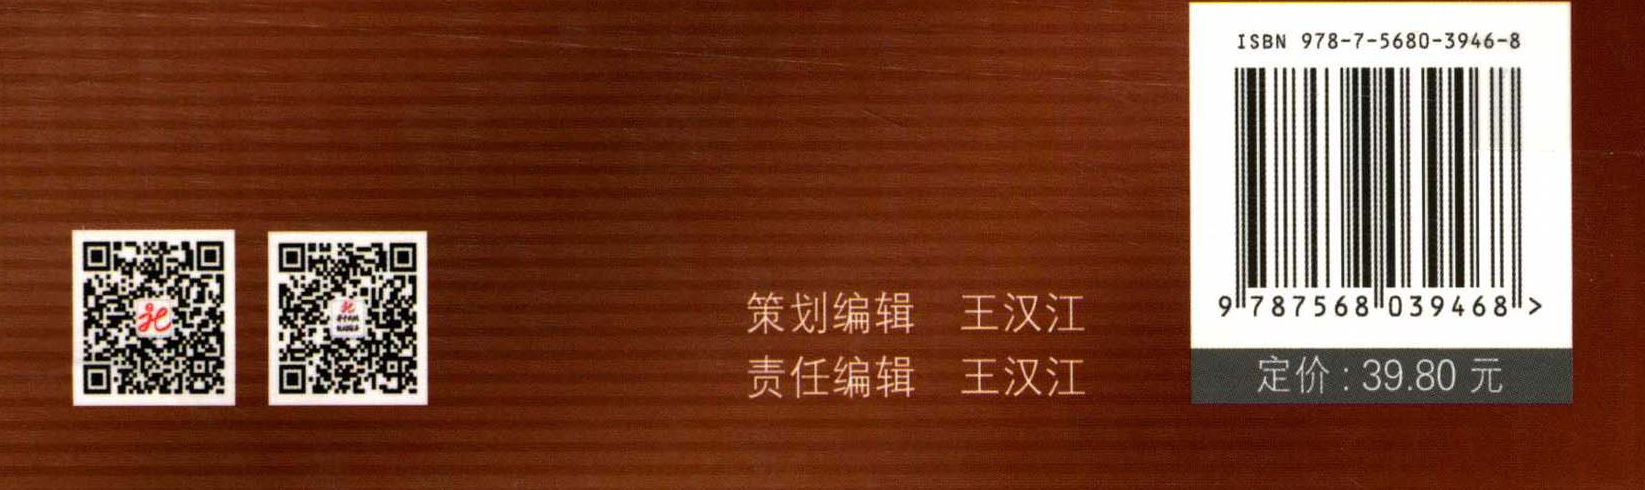
\includegraphics[width=0.85\linewidth,height=\textheight,keepaspectratio,alt={封底下方两个二维码、编辑姓名、ISBN、条码和定价，原扫描裁切}]{verified/assets/back/pdf-322-cover-bottom.png}

